\documentclass{../Common/Structure/doc_pdf}

\titleSubtitle{{\Huge\textit{Hypermedia project}}\\Prof. Franca Garzotto\\ \vspace{1cm}{\LARGE Usability report}}{Version 1.0.0}
\pageHeader{M.~Travaglini, F.~Di Febbo, F.~Zanoli}

\begin{document}
\titleToc

\chapter{Abstract}
This document aims to analyze and describe the usability characteristics of an application. Usability is a measure of "the effectiveness, efficiency and satisfaction with which specified users can achieve specified goals in particular environments" (ISO 9241-11).
The website to be inspected is (\url{www.tim.it})

\chapter{Introduction}
In the next chapter four scenarios are described. A scenario describes a user that tries to accomplish an objective, and the steps made by him/her. Each scenario is hence provided with a result section in which is described the evaluation of the heuristics of the pages visited by the user. Every member of this working group has performed an inspection of each page, the results have been discussed, and this document reports a wrap up of those results. The heuristics used for the analysis are the ones described by the MiLE (Milano-Lugano Evaluation Method) document.\\
The website evaluated is \url{www.tim.it}. This site provides services, products, promotions regarding in particular phone communication.
\vspace{1cm}
\begin{center}
	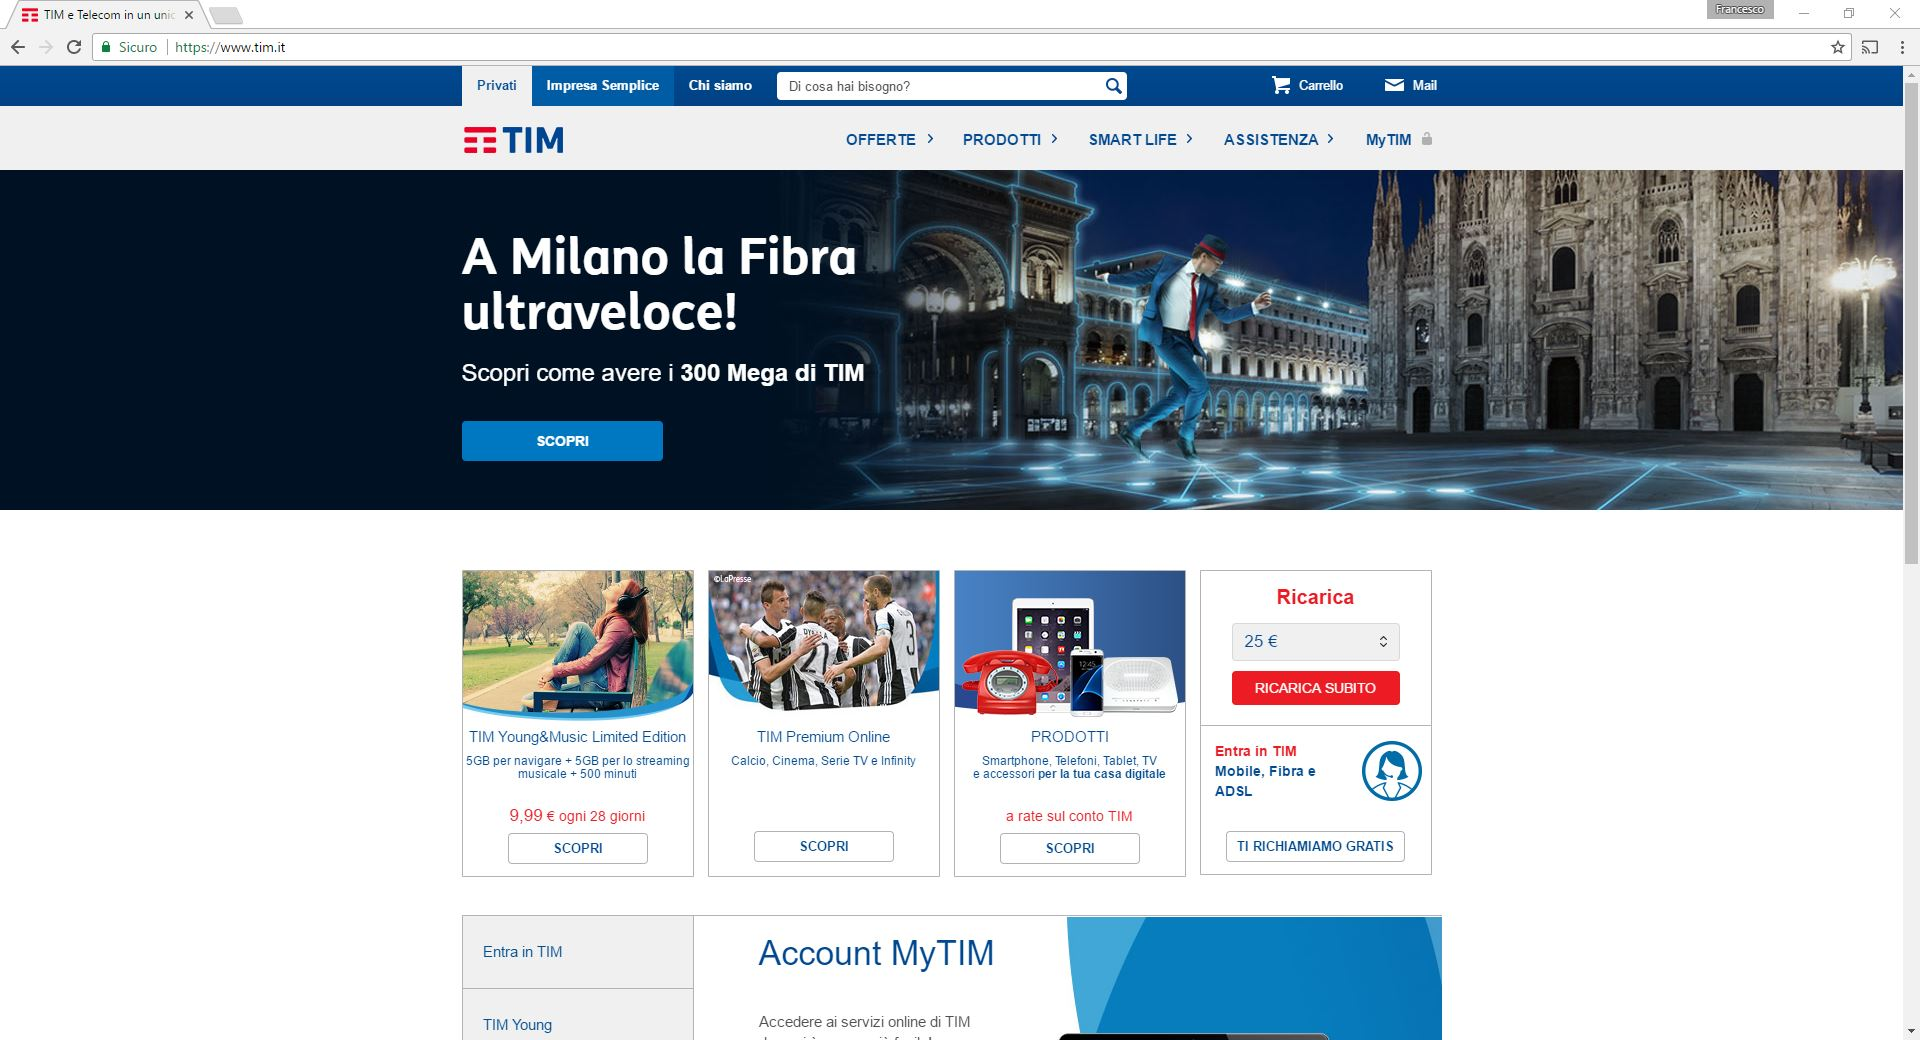
\includegraphics[width=\textwidth]{Screenshot/homepage.jpg}
\end{center}

\
\chapter{Scenarios}
\section{Scenario 1}
Alberto has to buy a new smartphone. He loves the services that his provider offers and he knows he can buy a new phone on its website.

\begin{enumerate}
	\item He goes on \url{www.tim.it}
	\item He clicks on "PRODOTTI" \url{www.tim.it/prodotti}
	\item In the smartphone section he can choose between smartphone or iPhone. He clicks on "iPhone" \url{www.tim.it/prodotti/smartphone-e-telefoni/iphone}
	\item Alberto sees that there are no promotions on iPhone so he goes back by clicking on "PRODOTTI"
	\item There is a promotion on Samsung Galaxy S8. He clicks on "SCOPRI" \url{www.tim.it/prodotti/smartphone-e-telefoni/samsung-galaxy-s8}
	\item He looks for the price and the specs. Alberto is interested and he wants to buy this phone. He clicks on "ACQUISTA". He is redirected on the ecommerce website of TIM and the purchase is continued through this site
\end{enumerate}

\subsection{Results}
\begin{enumerate}
	
%------------------------------------------------------------------------------------------------------
	
\item Report on \url{www.tim.it}	
	\paragraph*{Content heuristics \\ Text}
	\begin{itemize}
		\item accuracy: satisfied
		\item currency: \textcolor{red}{severely violated}\\the user cannot know if the page is updated
		\item coverage: satisfied
		\item content objectivity: satisfied
		\item authority: satisfied
		\item conciseness: satisfied		
	\end{itemize}
	
	\paragraph*{General communication quality}
	\begin{itemize}
		\item text errors: satisfied
		\item multimedia consistency: satisfied
	\end{itemize}

	\paragraph*{Navigation heuristics \\ Navigation within a topic}
	\begin{itemize}
		\item segmentation: n/a
	\end{itemize}	
	
	\paragraph*{Navigation within a transition}
	\begin{itemize}
		\item transition list: n/a
	\end{itemize}
	
	\paragraph*{Navigation within a group of topics}
	\begin{itemize}
		\item introduction list: n/a
		\item group navigation: n/a
	\end{itemize}
	
	\paragraph*{Backward navigation}
	\begin{itemize}
		\item go back: n/a
	\end{itemize}
	
	\paragraph*{Overall navigation}
	\begin{itemize}
		\item landmarks: satisfied\\
		they are well visible on the top-right corner of the website
		\item link consistency: satisfied
		\item orientation clues: satisfied
		\item orientation clues - topic: n/a
		\item group orientation clues: n/a
		\item transition orientation clues: n/a
	\end{itemize}	
	
	\paragraph*{Visual and semantic heuristics \\ Overall graphic design }
	\begin{itemize}
		\item visual identity: satisfied\\
		the palette represents the colors of the company logo
		\item chromatic code consistency: satisfied
		\item background contrast: satisfied
		\item font size: satisfied
		\item font color: satisfied
		\item font type: satisfied
		\item anchor identity: satisfied\\
		several links are wrapped in buttons 
		\item anchor states: satisfied\\
		anchors change states when the user hovers on them
		\item icon consistency: satisfied
	\end{itemize}
	
	\paragraph*{Page layout}
	\begin{itemize}
		\item visual proximity: satisfied
		\item layout conventions: satisfied
		\item semiotics: satisfied
	\end{itemize}	
	
	\paragraph*{Cognitive heuristics \\ Single page}
	\begin{itemize}
		\item information overload: \textcolor{orange}{partially violated}\\
		due to the number of services that the site offers, a novice could be overwhelmed by a lot of informations
	\end{itemize}	
	
	\paragraph*{Information architecture}
	\begin{itemize}
		\item classification adequacy within group of topics: n/a
		\item website mental map: satisfied
	\end{itemize}
\newpage
%------------------------------------------------------------------------------------------------------

\item Report on \url{www.tim.it/prodotti}

\begin{center}
	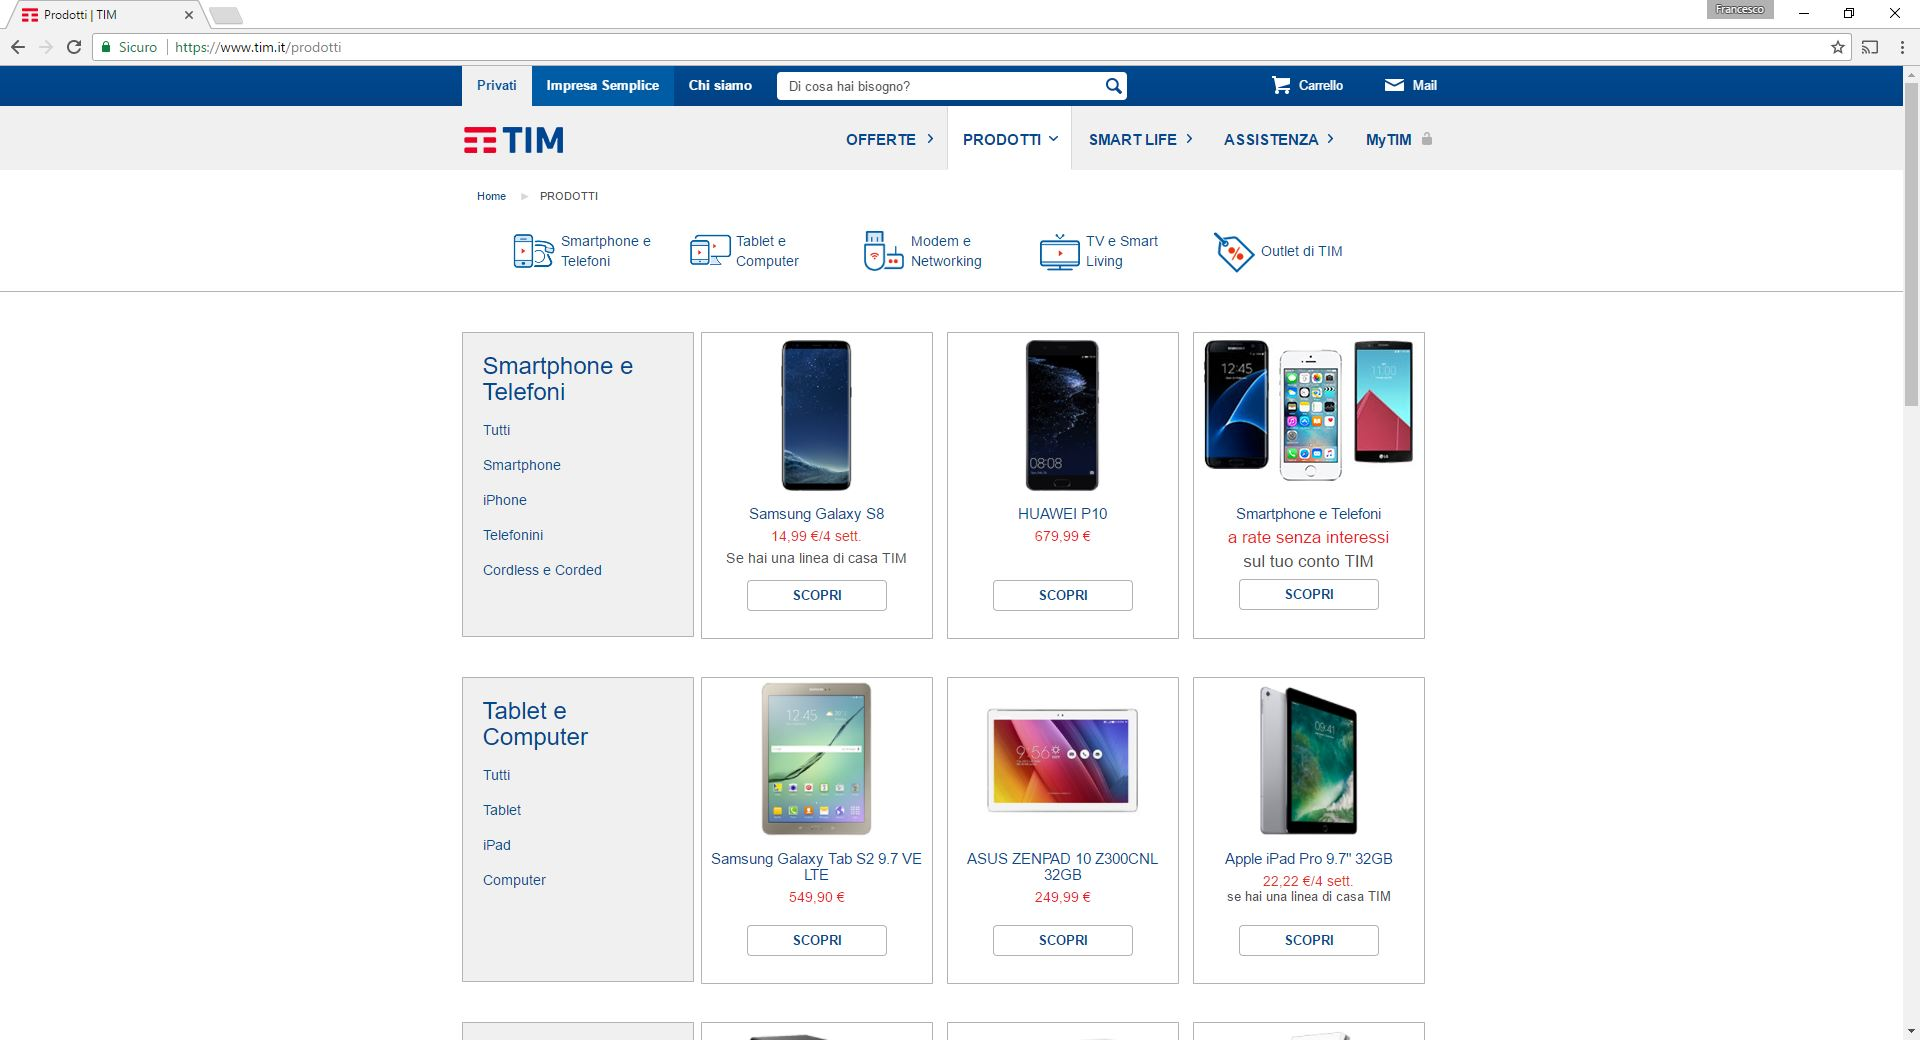
\includegraphics[width=\textwidth]{Screenshot/prodotti.jpg}
\end{center}
\vspace{1cm}

	\paragraph*{Content heuristics \\ Text}
	\begin{itemize}
		\item accuracy: satisfied
		\item currency: \textcolor{red}{severely violated}\\the user cannot know if the page is updated
		\item coverage: satisfied
		\item content objectivity: satisfied
		\item authority: satisfied
		\item conciseness: satisfied		
	\end{itemize}

	\paragraph*{General communication quality}
	\begin{itemize}
		\item text errors: satisfied
		\item multimedia consistency: satisfied
	\end{itemize}

	\paragraph*{Navigation heuristics \\ Navigation within a topic}
	\begin{itemize}
		\item segmentation: n/a
	\end{itemize}	
	
	\paragraph*{Navigation within a transition}
	\begin{itemize}
		\item transition list: n/a
	\end{itemize}
	
	\paragraph*{Navigation within a group of topics}
	\begin{itemize}
		\item introduction list: satisfied\\
		this site identifies several groups of topics ("Smartphone e Telefoni", "Tablet e Computer"...)
		\item group navigation: n/a
	\end{itemize}

	\paragraph*{Backward navigation}
	\begin{itemize}
		\item go back: \textcolor {orange}{partially violated}\\
		there isn't a "go back" functionality but the user can exploit the TIM logo to return to the homepage or select a position in the website structure path (Home $\triangleright$ PRODOTTI)
	\end{itemize}
	
	\paragraph*{Overall navigation}
	\begin{itemize}
		\item landmarks: satisfied\\
		they are well visible on the top-right corner of the website
		\item link consistency: satisfied
		\item orientation clues: satisfied\\
		under the logo there is a site structure path
		\item orientation clues - topic: n/a
		\item group orientation clues: n/a
		\item transition orientation clues: n/a
	\end{itemize}	
	
	\paragraph*{Visual and semantic heuristics \\ Overall graphic design }
	\begin{itemize}
		\item visual identity: satisfied
		\item chromatic code consistency: satisfied
		\item background contrast: satisfied
		\item font size: satisfied
		\item font color: satisfied
		\item font type: satisfied
		\item anchor identity: satisfied
		\item anchor states: satisfied
		\item icon consistency: satisfied
	\end{itemize}
	
	\paragraph*{Page layout}
	\begin{itemize}
		\item visual proximity: satisfied
		\item layout conventions: satisfied
		\item semiotics: satisfied
	\end{itemize}	
	
	\paragraph*{Cognitive heuristics \\ Single page}
	\begin{itemize}
		\item information overload: satisfied
	\end{itemize}	
	
	\paragraph*{Information architecture}
	\begin{itemize}
		\item classification adequacy within group of topics: n/a
		\item website mental map: satisfied
	\end{itemize}

%------------------------------------------------------------------------------------------------------

\item Report on \url{www.tim.it/prodotti/smartphone-e-telefoni/iphone}

\begin{center}
	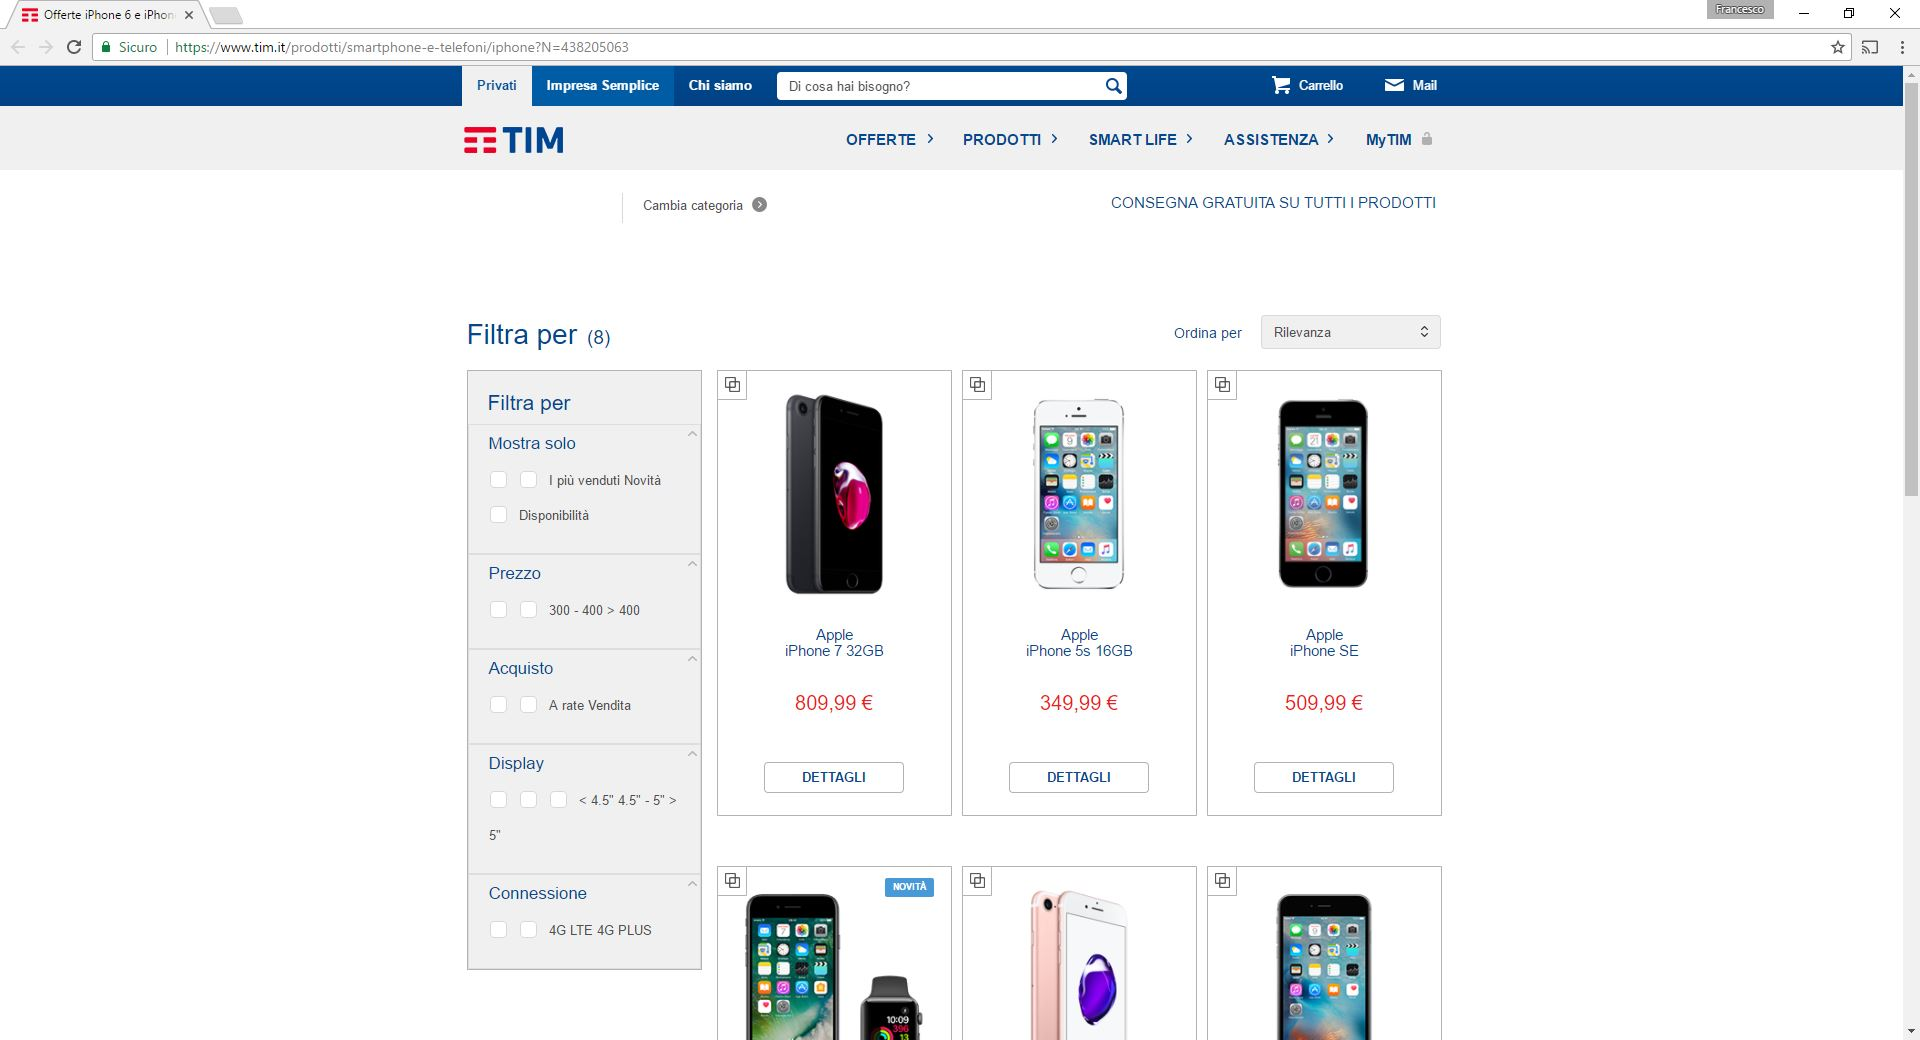
\includegraphics[width=\textwidth]{Screenshot/iphone.jpg}
\end{center}
\vspace{1cm}

	\paragraph*{Content heuristics \\ Text}
	\begin{itemize}
		\item accuracy: satisfied
		\item currency: \textcolor{red}{severely violated}\\the user cannot know if the page is updated
		\item coverage: satisfied
		\item content objectivity: satisfied
		\item authority: satisfied
		\item conciseness: satisfied		
	\end{itemize}
	
	\paragraph*{General communication quality}
	\begin{itemize}
		\item text errors: satisfied
		\item multimedia consistency: satisfied
	\end{itemize}
	
	\paragraph*{Navigation heuristics \\ Navigation within a topic}
	\begin{itemize}
		\item segmentation: n/a
	\end{itemize}	
	
	\paragraph*{Navigation within a transition}
	\begin{itemize}
		\item transition list: n/a
	\end{itemize}
	
	\paragraph*{Navigation within a group of topics}
	\begin{itemize}
		\item introduction list: n/a
		\item group navigation: satisfied\\
		from this page it is possible to reach every item of this group of topics
	\end{itemize}
	
	\paragraph*{Backward navigation}
	\begin{itemize}
		\item go back: \textcolor{red}{severely violated}\\
		there is no "go back" functionality, the user can go to the homepage through the TIM logo or repeat the steps by clicking "PRODOTTI"
	\end{itemize}
	
	\paragraph*{Overall navigation}
	\begin{itemize}
		\item landmarks: satisfied\\
		they are well visible on the top-right corner of the website 
		\item link consistency: satisfied
		\item orientation clues: \textcolor{red}{severely violated}\\
		the user cannot know where he/she is, there are no title nor path
		\item orientation clues - topic: n/a
		\item group orientation clues: \textcolor{red}{severely violated}\\
		the user cannot know which group of topics he/she is visiting ("Smartphone e Telefoni/iPhone")
		\item transition orientation clues: n/a
	\end{itemize}	
	
	\paragraph*{Visual and semantic heuristics \\ Overall graphic design }
	\begin{itemize}
		\item visual identity: satisfied
		\item chromatic code consistency: satisfied
		\item background contrast: satisfied
		\item font size: satisfied
		\item font color: satisfied
		\item font type: satisfied
		\item anchor identity: satisfied
		\item anchor states: satisfied
		\item icon consistency: satisfied
	\end{itemize}
	
	\paragraph*{Page layout}
	\begin{itemize}
		\item visual proximity: satisfied
		\item layout conventions: satisfied
		\item semiotics: satisfied
	\end{itemize}	
	
	\paragraph*{Cognitive heuristics \\ Single page}
	\begin{itemize}
		\item information overload: satisfied
	\end{itemize}	

	\paragraph*{Information architecture}
	\begin{itemize}
		\item classification adequacy within group of topics: satisfied
		\item website mental map: satisfied
	\end{itemize}

\newpage

%------------------------------------------------------------------------------------------------------

\item Report on \url{www.tim.it/prodotti/smartphone-e-telefoni/samsung-galaxy-s8}

\begin{center}
	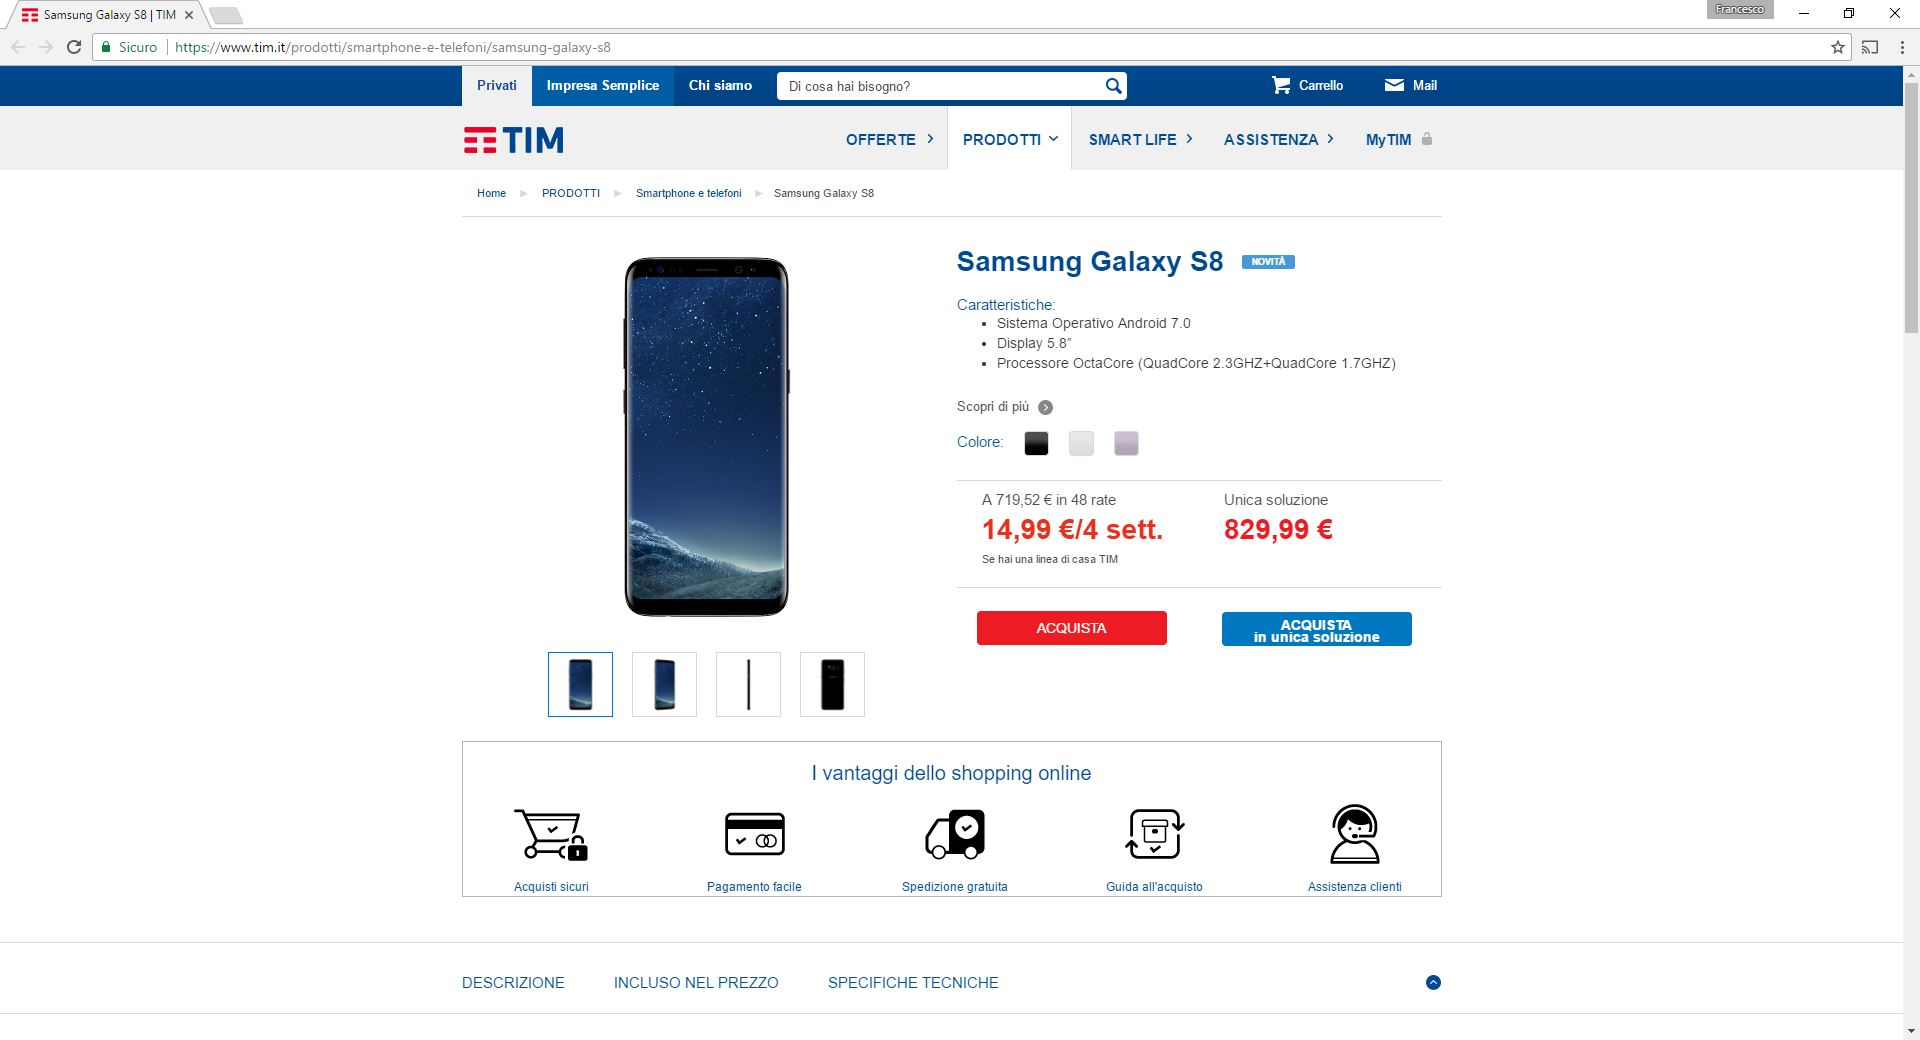
\includegraphics[width=\textwidth]{Screenshot/galaxys8.jpg}
\end{center}
\vspace{1cm}

	\paragraph*{Content heuristics \\ Text}
	\begin{itemize}
		\item accuracy: satisfied
		\item currency: \textcolor{red}{severely violated}\\the user cannot know if the page is updated
		\item coverage: satisfied
		\item content objectivity: satisfied
		\item authority: satisfied
		\item conciseness: satisfied		
	\end{itemize}

	\paragraph*{General communication quality}
	\begin{itemize}
		\item text errors: satisfied
		\item multimedia consistency: satisfied
	\end{itemize}

	\paragraph*{Navigation heuristics \\ Navigation within a topic}
	\begin{itemize}
		\item segmentation: satisfied\\
		the information of the topic are organized in sub-sections on the same page
	\end{itemize}	

	\paragraph*{Navigation within a transition}
	\begin{itemize}
		\item transition list: satisfied\\
		there are links related to other topics ("I vantaggi dello shopping online")
	\end{itemize}

	\paragraph*{Navigation within a group of topics}
	\begin{itemize}
		\item introduction list: n/a
		\item group navigation: \textcolor{orange}{partially violated}\\
		the user can reach the group by the site structure path but he/she can't reach items related to the group
	\end{itemize}

	\paragraph*{Backward navigation}
	\begin{itemize}
		\item go back: \textcolor{orange}{partially violated}\\
		there isn't a "go back" functionality but the user can exploit the TIM logo to return to the homepage or select a position in the website structure path (Home $\triangleright$ PRODOTTI $\triangleright$ Smartphone e Telefoni $\triangleright$ Samsung Galaxy S8)
	\end{itemize}

	\paragraph*{Overall navigation}
	\begin{itemize}
		\item landmarks: satisfied\\
		they are well visible on the top-right corner of the website
		\item link consistency: satisfied
		\item orientation clues: satisfied\\
		under the logo there is a site structure path
		\item orientation clues - topic: satisfied\\
		the user knows the subsection he/she is visiting. When the user navigate through the site, the section's labels are well visible on top of the page
		\item group orientation clues: satisfied
		\item transition orientation clues: satisfied
	\end{itemize}	

	\paragraph*{Visual and semantic heuristics \\ Overall graphic design }
	\begin{itemize}
		\item visual identity: satisfied
		\item chromatic code consistency: satisfied
		\item background contrast: satisfied
		\item font size: satisfied
		\item font color: satisfied
		\item font type: satisfied
		\item anchor identity: satisfied
		\item anchor states: satisfied
		\item icon consistency: satisfied
	\end{itemize}

	\paragraph*{Page layout}
	\begin{itemize}
		\item visual proximity: satisfied
		\item layout conventions: satisfied
		\item semiotics: satisfied
	\end{itemize}

	\paragraph*{Cognitive heuristics \\ Single page}
	\begin{itemize}
		\item information overload: satisfied
	\end{itemize}	

	\paragraph*{Information architecture}
	\begin{itemize}
		\item classification adequacy within group of topics: n/a
		\item website mental map: satisfied
	\end{itemize}
	\end{enumerate}
\section{Scenario 2}
Barbara has moved to a new home ad now she needs for a new telephone number and an internet connection.

\begin{enumerate}
	\item She goes on \url{www.tim.it}
	\item She clicks on "Verifica la copertura 4G, Fibra e ADSL" \url{www.tim.it/verifica-copertura#tab-verifica-fisso}
	\item She enters her address information in the form and she clicks "VERIFICA". Her home is reached by fyber and adsl connection by TIM so she decides to look for a promotion. She clicks on TIM logo to return to the homepage.
	\item She overs the mouse on "OFFERTE" and clicks on "Fisso" \url{www.tim.it/offerte/fisso}
	\item She clicks on "TIM SMART FIBRA PLUS" \url{www.tim.it/offerte/fisso/internet-voce-e-timvision/fibra/tim-smart-fibra-plus}
	\item On the left side she clicks on "Costi". The costs look good so she decides to choose this promotion. Barbara clicks on "ATTIVA". The website redirects her to the ecommerce website of TIM and she continues from here.
\end{enumerate}

\subsection{Results}
\begin{enumerate}
	
%------------------------------------------------------------------------------------------------------
	
\item Report on \url{www.tim.it/verifica-copertura#tab-verifica-fisso}	
	\paragraph*{Content heuristics \\ Text}
	\begin{itemize}
		\item accuracy: satisfied
		\item currency: \textcolor{red}{severely violated}\\the user cannot know if the page is updated
		\item coverage: satisfied
		\item content objectivity: n/a
		\item authority: satisfied
		\item conciseness: satisfied		
	\end{itemize}
	
	\paragraph*{General communication quality}
	\begin{itemize}
		\item text errors: satisfied
		\item multimedia consistency: satisfied
	\end{itemize}

	\paragraph*{Navigation heuristics \\ Navigation within a topic}
	\begin{itemize}
		\item segmentation: n/a
	\end{itemize}	
	
	\paragraph*{Navigation within a transition}
	\begin{itemize}
		\item transition list: n/a
	\end{itemize}
	
	\paragraph*{Navigation within a group of topics}
	\begin{itemize}
		\item introduction list: n/a
		\item group navigation: n/a
	\end{itemize}
	
	\paragraph*{Backward navigation}
	\begin{itemize}
		\item go back: \textcolor {orange}{partially violated}\\
		there isn't a "go back" functionality but the user can exploit the TIM logo to return to the homepage or select a position in the website structure path (Home $\triangleright$ Verifica copertura)
	\end{itemize}
	
	\paragraph*{Overall navigation}
	\begin{itemize}
		\item landmarks: satisfied
		\item link consistency: satisfied
		\item orientation clues: satisfied
		\item orientation clues - topic: n/a
		\item group orientation clues: n/a
		\item transition orientation clues: n/a
	\end{itemize}	
	
	\paragraph*{Visual and semantic heuristics \\ Overall graphic design }
	\begin{itemize}
		\item visual identity: satisfied\\
		the palette represents the colors of the company logo
		\item chromatic code consistency: satisfied
		\item background contrast: satisfied
		\item font size: satisfied
		\item font colour: satisfied
		\item font type: satisfied
		\item anchor identity: satisfied
		\item anchor states: satisfied
		\item icon consistency: satisfied
	\end{itemize}
	
	\paragraph*{Page layout}
	\begin{itemize}
		\item visual proximity: satisfied
		\item layout conventions: satisfied
		\item semiotics: satisfied
	\end{itemize}	
	
	\paragraph*{Cognitive heuristics \\ Single page}
	\begin{itemize}
		\item information overload: satisfied
	\end{itemize}	
	
	\paragraph*{Information architecture}
	\begin{itemize}
		\item classification adequacy within group of topics: satisfied
		\item website mental map: satisfied
	\end{itemize}

%------------------------------------------------------------------------------------------------------

\item Report on \url{www.tim.it/offerte/fisso}
	\paragraph*{Content heuristics \\ Text}
	\begin{itemize}
		\item accuracy: satisfied
		\item currency: \textcolor{orange}{partially violated}\\
		the user knows that the site is updated through the promotions that are limited for the current period
		\item coverage: satisfied
		\item content objectivity: n/a
		\item authority: satisfied
		\item conciseness: satisfied		
	\end{itemize}

	\paragraph*{General communication quality}
	\begin{itemize}
		\item text errors: satisfied
		\item multimedia consistency: satisfied
	\end{itemize}

	\paragraph*{Navigation heuristics \\ Navigation within a topic}
	\begin{itemize}
		\item segmentation: n/a
	\end{itemize}	
	
	\paragraph*{Navigation within a transition}
	\begin{itemize}
		\item transition list: n/a
	\end{itemize}
	
	\paragraph*{Navigation within a group of topics}
	\begin{itemize}
		\item introduction list: satisfied
		\item group navigation: satisfied
	\end{itemize}

	\paragraph*{Backward navigation}
	\begin{itemize}
		\item go back: \textcolor {orange}{partially violated}\\
		there isn't a "go back" functionality but the user can exploit the TIM logo to return to the homepage or select a position in the website structure path (Home $\triangleright$ OFFERTE $\triangleright$ Fisso)
	\end{itemize}
	
	\paragraph*{Overall navigation}
	\begin{itemize}
		\item landmarks: satisfied
		\item link consistency: satisfied
		\item orientation clues: satisfied
		\item orientation clues - topic: n/a
		\item group orientation clues: satisfied
		\item transition orientation clues: n/a
	\end{itemize}	
	
	\paragraph*{Visual and semantic heuristics \\ Overall graphic design }
	\begin{itemize}
		\item visual identity: satisfied
		\item chromatic code consistency: satisfied
		\item background contrast:satisfied
		\item font size: satisfied
		\item font colour: satisfied
		\item font type: satisfied
		\item anchor identity: satisfied
		\item anchor states: satisfied
		\item icon consistency: satisfied
	\end{itemize}
	
	\paragraph*{Page layout}
	\begin{itemize}
		\item visual proximity: satisfied
		\item layout conventions: satisfied
		\item semiotics: satisfied
	\end{itemize}	
	
	\paragraph*{Cognitive heuristics \\ Single page}
	\begin{itemize}
		\item information overload: satisfied
	\end{itemize}	
	
	\paragraph*{Information architecture}
	\begin{itemize}
		\item classification adequacy within group of topics: satisfied
		\item website mental map: satisfied
	\end{itemize}

%------------------------------------------------------------------------------------------------------

\item Report on \url{www.tim.it/offerte/fisso/internet-voce-e-timvision/fibra/tim-smart-fibra-plus}
	\paragraph*{Content heuristics \\ Text}
	\begin{itemize}
		\item accuracy: satisfied
		\item currency:  \textcolor{orange}{partially violated}\\
		the user knows that the site is updated through the promotions that are limited for the current period
		\item coverage: satisfied
		\item content objectivity: satisfied
		\item authority: satisfied
		\item conciseness: satisfied		
	\end{itemize}

	\paragraph*{General communication quality}
	\begin{itemize}
		\item text errors: satisfied
		\item multimedia consistency: satisfied
	\end{itemize}

	\paragraph*{Navigation heuristics \\ Navigation within a topic}
	\begin{itemize}
		\item segmentation: satisfied\\
		the information of the topic are organized in sub-sections (accessible on the left side) on the same page
	\end{itemize}	

	\paragraph*{Navigation within a transition}
	\begin{itemize}
		\item transition list: satisfied
	\end{itemize}

	\paragraph*{Navigation within a group of topics}
	\begin{itemize}
		\item introduction list: n/a
		\item group navigation: n/a
	\end{itemize}

	\paragraph*{Backward navigation}
	\begin{itemize}
		\item go back: \textcolor {orange}{partially violated}\\
		there isn't a "go back" functionality but the user can exploit the TIM logo to return to the homepage or select a position in the website structure path (Home $\triangleright$ OFFERTE $\triangleright$ Fisso $\triangleright$ Internet Voce e TIMvision $\triangleright$ Fibra $\triangleright$ TIM SMART FIBRA PLUS)
	\end{itemize}

	\paragraph*{Overall navigation}
	\begin{itemize}
		\item landmarks: satisfied
		\item link consistency: satisfied
		\item orientation clues: satisfied
		\item orientation clues - topic: satisfied
		\item group orientation clues: satisfied
		\item transition orientation clues: satisfied
	\end{itemize}	

	\paragraph*{Visual and semantic heuristics \\ Overall graphic design }
	\begin{itemize}
		\item visual identity: satisfied (the colors represents the logo of the company)
		\item chromatic code consistency: satisfied
		\item background contrast:satisfied
		\item font size: satisfied
		\item font colour: satisfied
		\item font type: satisfied
		\item anchor identity: satisfied
		\item anchor states: satisfied
		\item icon consistency: satisfied
	\end{itemize}

	\paragraph*{Page layout}
	\begin{itemize}
		\item visual proximity: satisfied
		\item layout conventions: satisfied
		\item semiotics: satisfied
	\end{itemize}

	\paragraph*{Cognitive heuristics \\ Single page}
	\begin{itemize}
		\item information overload: satisfied
	\end{itemize}	

	\paragraph*{Information architecture}
	\begin{itemize}
		\item classification adequacy within group of topics: satisfied
		\item website mental map: satisfied
	\end{itemize}
	\end{enumerate}
\section{Scenario 3}
Summer is coming. Chiara wants to be in shape for the swimsuit season. She heard about the Smart Life services of TIM so she checks on their website.

\begin{enumerate}
	\item She goes on \url{www.tim.it}
	\item He clicks on "SMART LIFE" \url{www.tim.it/smart-life}
	\item She scrolls through the categories and she clicks on "Salute e benessere" \url{www.tim.it/smart-life/salute-benessere}
	\item She looks for products. She clicks on "Loop H7 HR" then on "SCOPRI I DETTAGLI" \url{www.tim.it/polar-loop-activity-tracker}
	\item She likes the product but she wants to look for other. She can't go back with navigation so she over the mouse on "SMART LIFE" and clicks on "Salute e benessere"
	\item Now she clicks on "Samsung Galaxy Gear Fit" then on "SCOPRI I DETTAGLI" \url{https://www.tim.it/prodotti/tv-e-smart-living/samsung-gear-fit}
	\item Chiara prefers this one. She looks for the specs and then clicks on "ACQUISTA". She is redirected to ecommerce website of TIM. She continues from here.
\end{enumerate}

\subsection{Results}
\begin{enumerate}
	
%------------------------------------------------------------------------------------------------------
	
\item Report on \url{www.tim.it/smart-life}

\begin{center}
	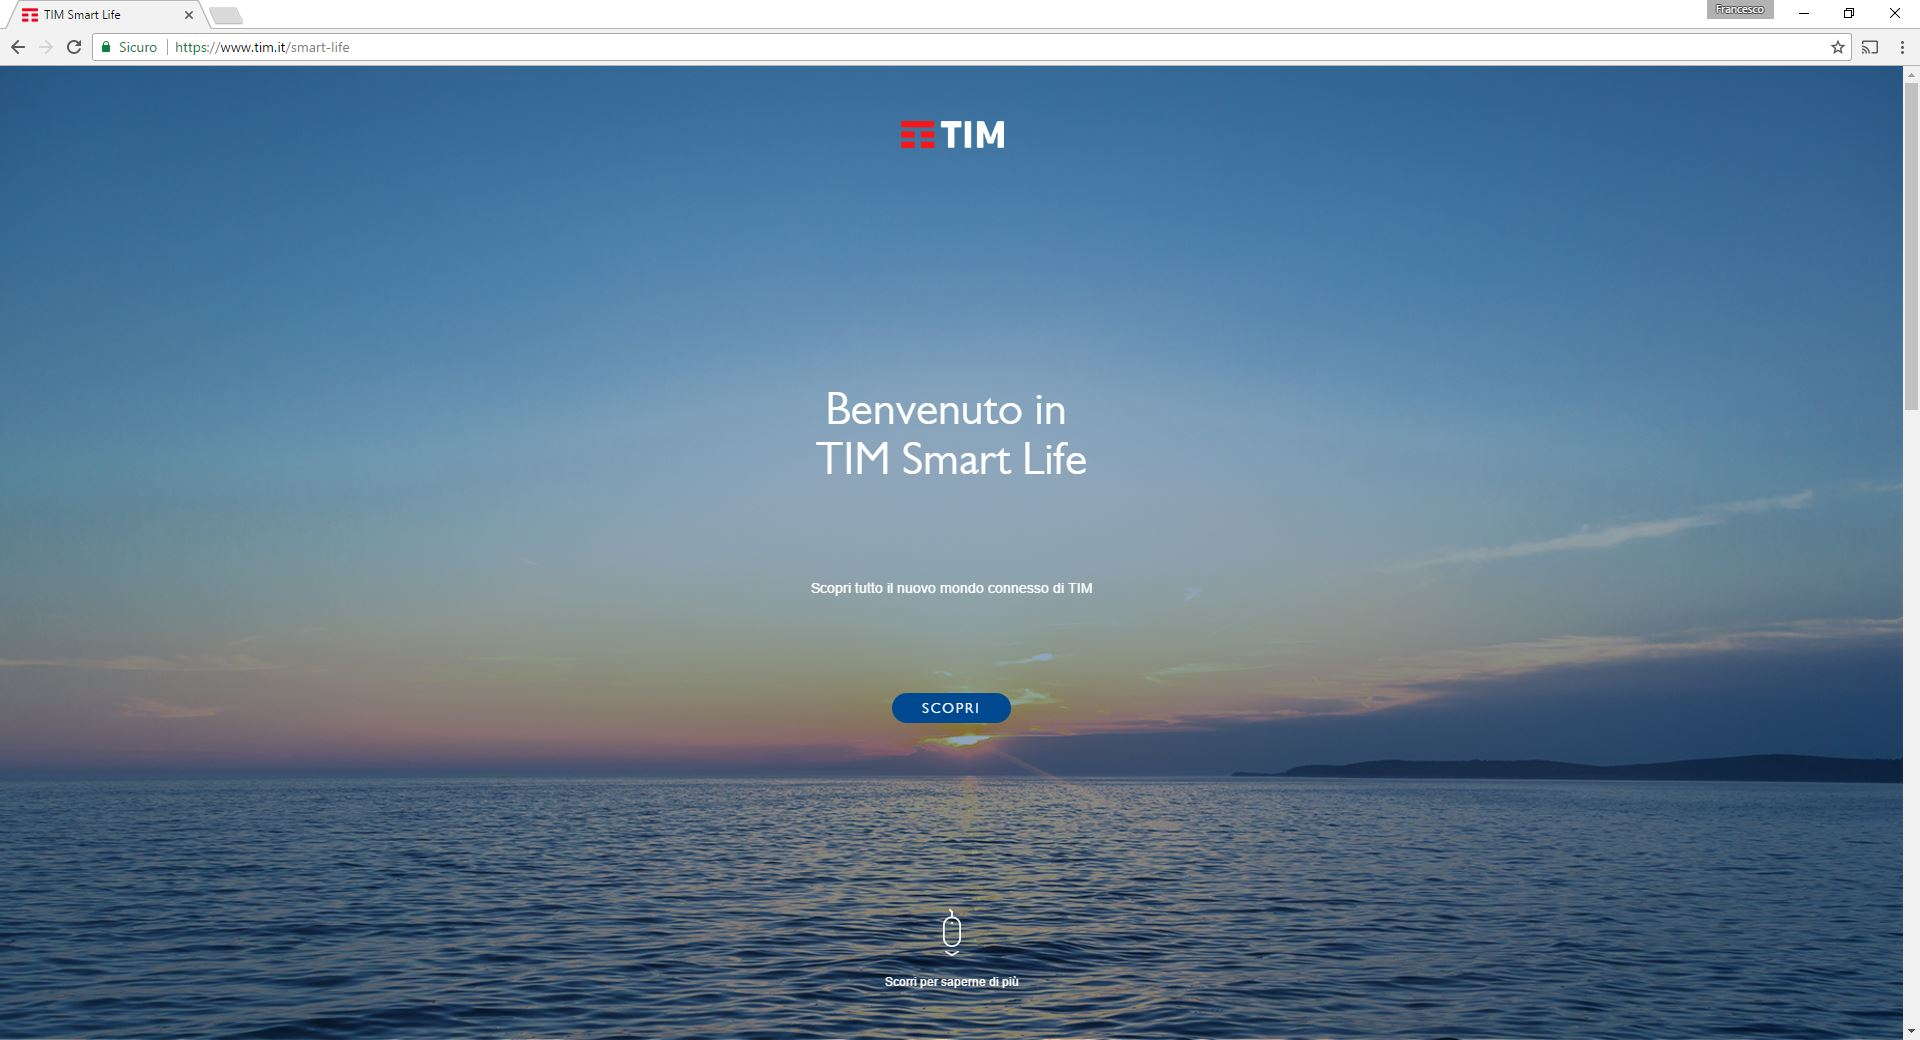
\includegraphics[width=\textwidth]{Screenshot/smartlife1.jpg}
\end{center}
\begin{center}
	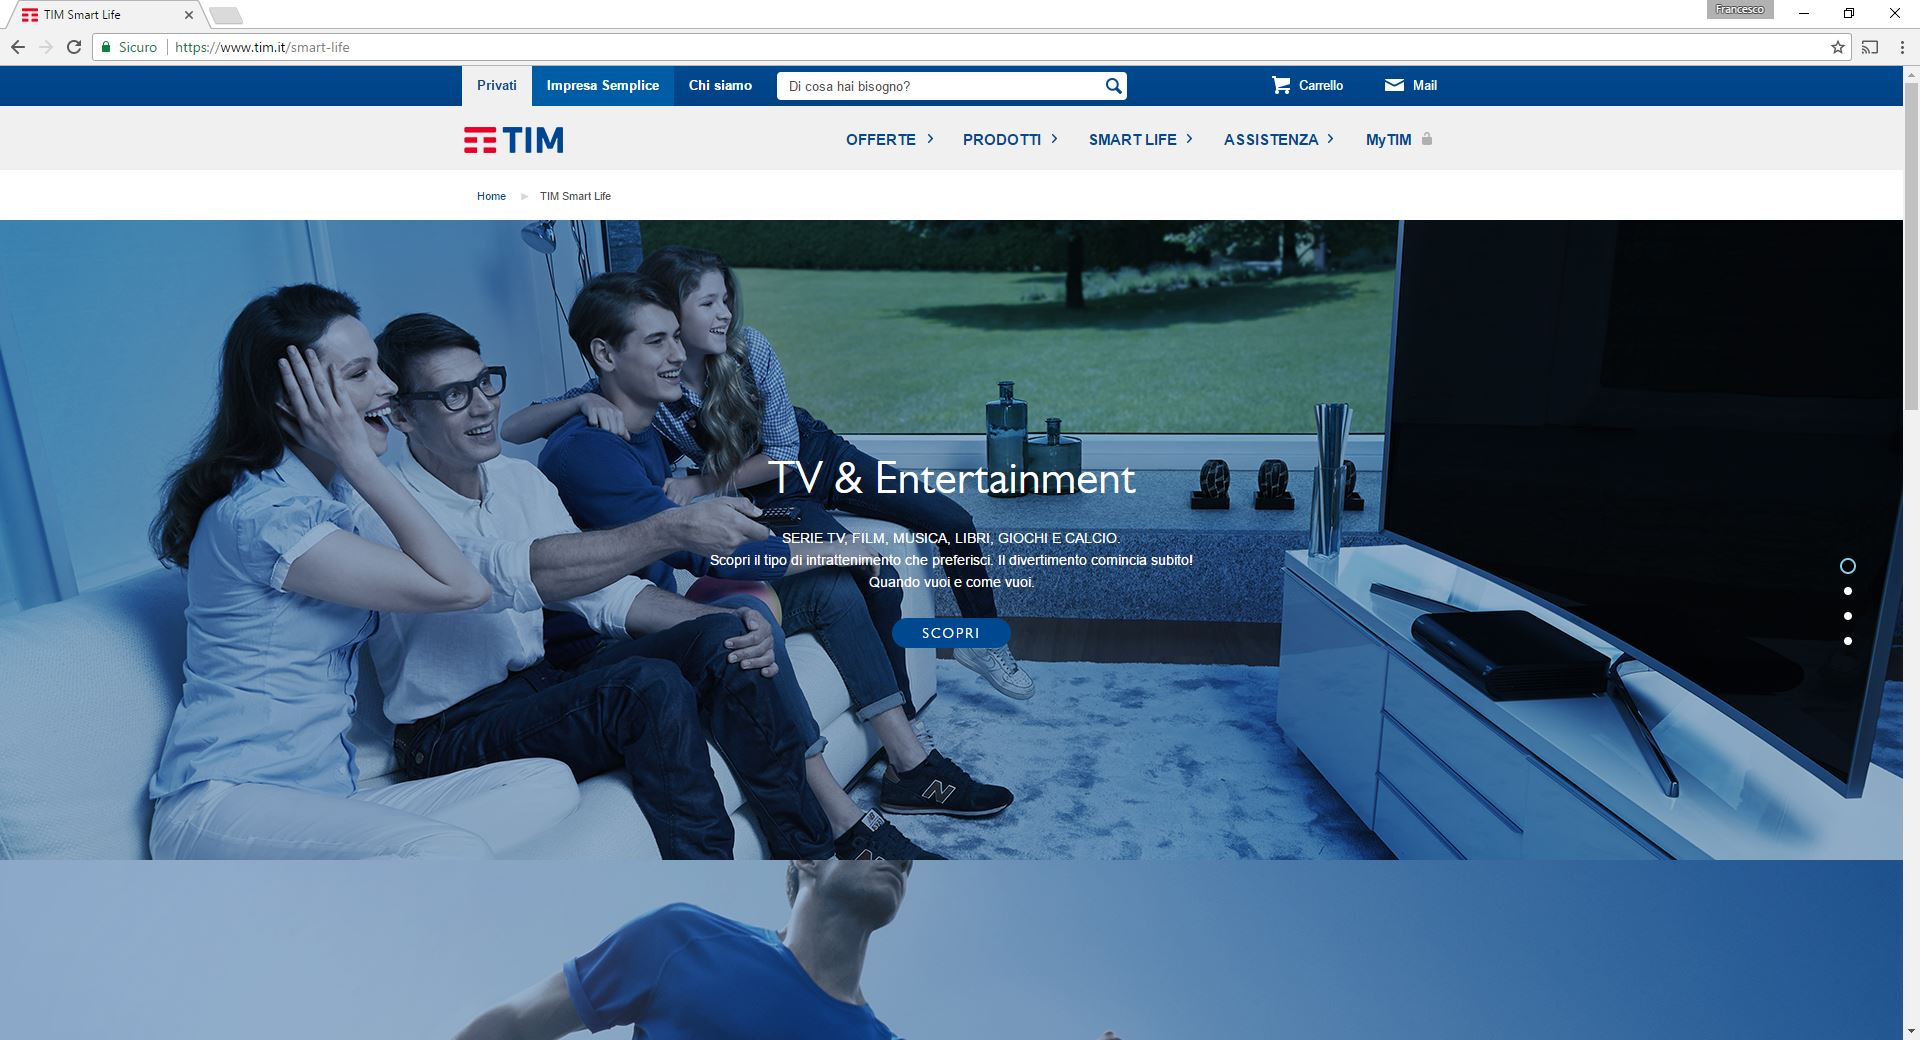
\includegraphics[width=\textwidth]{Screenshot/smartlife2.jpg}
\end{center}
\vspace{1cm}

	\paragraph*{Content heuristics \\ Text}
	\begin{itemize}
		\item accuracy: satisfied
		\item currency: \textcolor{red}{severely violated}\\
		the user cannot know if the page is updated
		\item coverage: satisfied
		\item content objectivity: satisfied
		\item authority: satisfied
		\item conciseness: satisfied		
	\end{itemize}
	
	\paragraph*{General communication quality}
	\begin{itemize}
		\item text errors: satisfied
		\item multimedia consistency: satisfied
	\end{itemize}

	\paragraph*{Navigation heuristics \\ Navigation within a topic}
	\begin{itemize}
		\item segmentation: n/a
	\end{itemize}	
	
	\paragraph*{Navigation within a transition}
	\begin{itemize}
		\item transition list: n/a
	\end{itemize}
	
	\paragraph*{Navigation within a group of topics}
	\begin{itemize}
		\item introduction list: satisfied
		\item group navigation: satisfied
	\end{itemize}
	
	\paragraph*{Backward navigation}
	\begin{itemize}
		\item go back: \textcolor {orange}{partially violated}\\
		there isn't a "go back" functionality but the user can exploit the TIM logo to return to the homepage or select a position in the website structure path (Home $\triangleright$ TIM Smart Life)
	\end{itemize}
	
	\paragraph*{Overall navigation}
	\begin{itemize}
		\item landmarks: satisfied
		\item link consistency: satisfied
		\item orientation clues: satisfied
		\item orientation clues - topic: n/a
		\item group orientation clues: n/a
		\item transition orientation clues: n/a
	\end{itemize}	
	
	\paragraph*{Visual and semantic heuristics \\ Overall graphic design }
	\begin{itemize}
		\item visual identity: satisfied\\
		the palette represents the colors of the company logo
		\item chromatic code consistency: satisfied
		\item background contrast:satisfied
		\item font size: satisfied
		\item font colour: satisfied
		\item font type: satisfied
		\item anchor identity: satisfied
		\item anchor states: satisfied
		\item icon consistency: satisfied
	\end{itemize}
	
	\paragraph*{Page layout}
	\begin{itemize}
		\item visual proximity: satisfied
		\item layout conventions: satisfied
		\item semiotics: satisfied
	\end{itemize}	
	
	\paragraph*{Cognitive heuristics \\ Single page}
	\begin{itemize}
		\item information overload: satisfied
	\end{itemize}	
	
	\paragraph*{Information architecture}
	\begin{itemize}
		\item classification adequacy within group of topics: satisfied
		\item website mental map: satisfied
	\end{itemize}
\newpage

%------------------------------------------------------------------------------------------------------

\item Report on \url{www.tim.it/smart-life/salute-benessere}

\begin{center}
	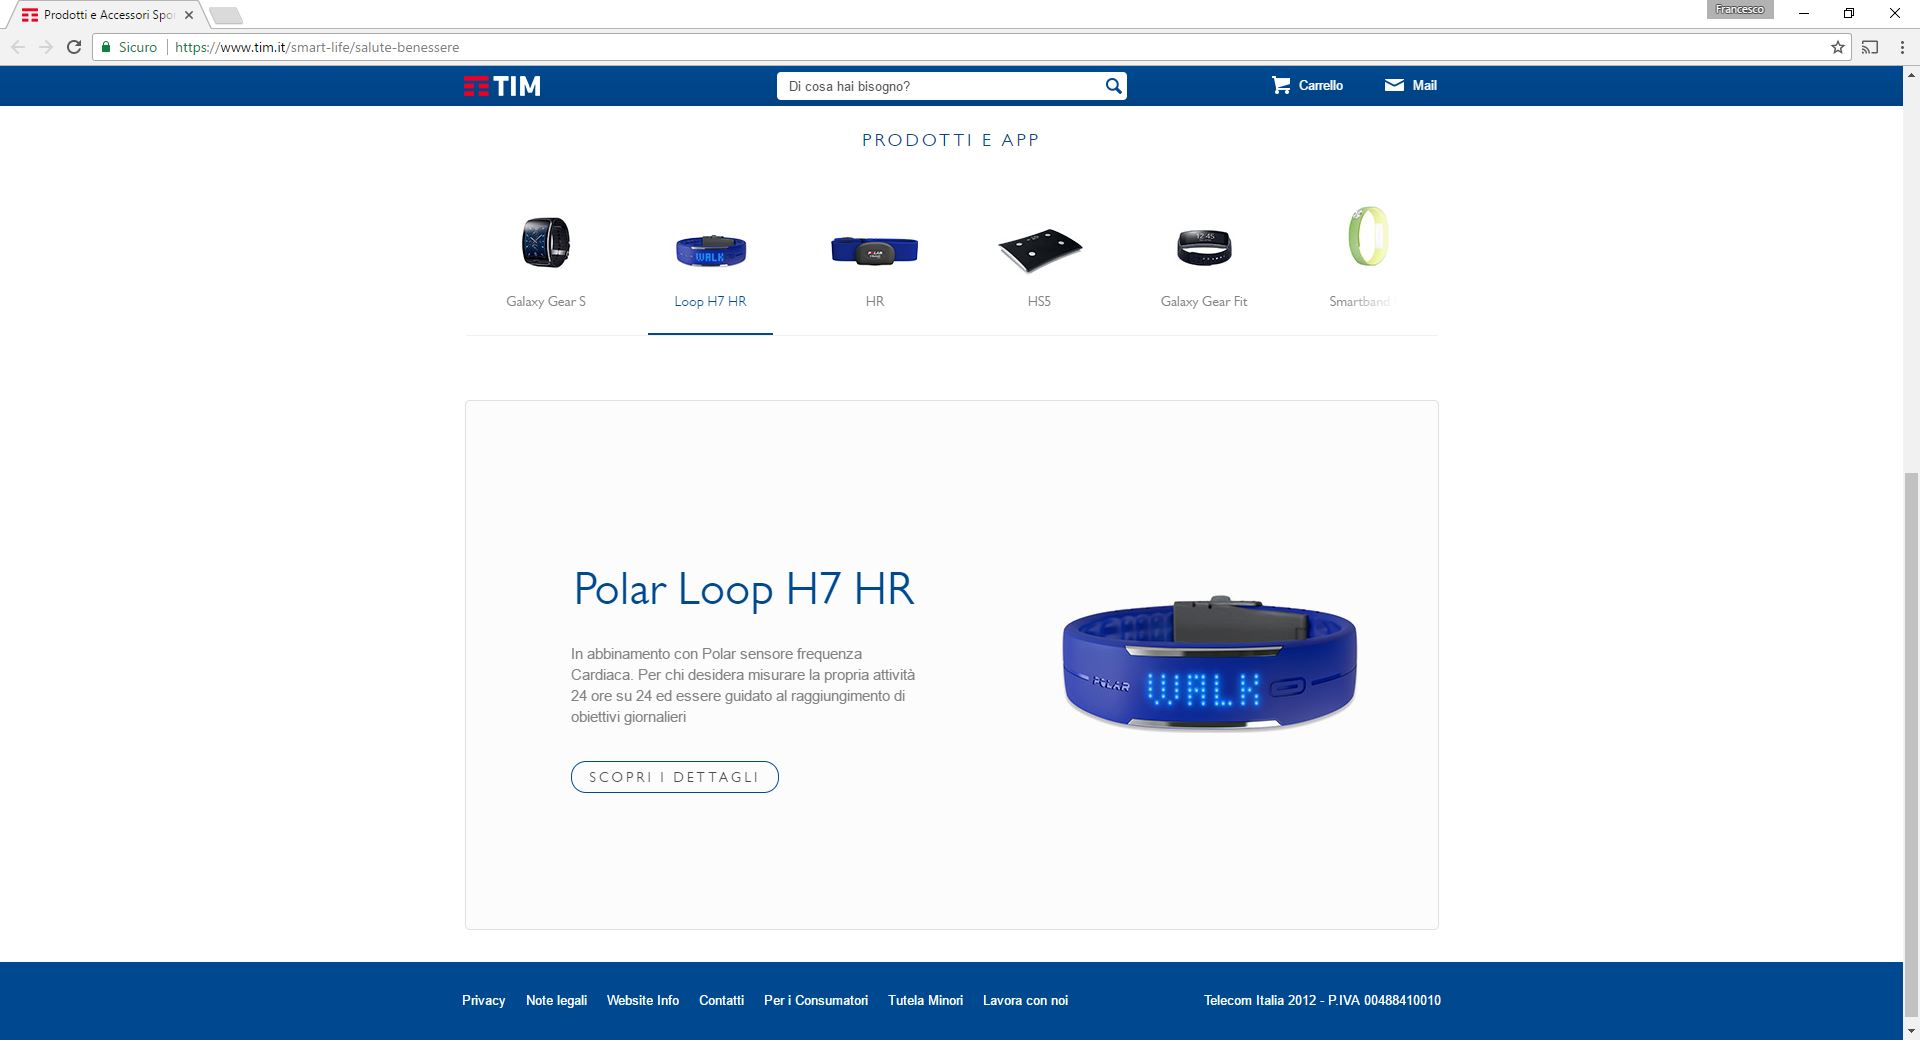
\includegraphics[width=\textwidth]{Screenshot/salute.jpg}
\end{center}
\vspace{1cm}

	\paragraph*{Content heuristics \\ Text}
	\begin{itemize}
		\item accuracy: satisfied
		\item currency: \textcolor{red}{severely violated}\\
		the user cannot know if the page is updated
		\item coverage: satisfied
		\item content objectivity: satisfied
		\item authority: satisfied
		\item conciseness: satisfied		
	\end{itemize}

	\paragraph*{General communication quality}
	\begin{itemize}
		\item text errors: satisfied
		\item multimedia consistency: satisfied
	\end{itemize}

	\paragraph*{Navigation heuristics \\ Navigation within a topic}
	\begin{itemize}
		\item segmentation: n/a
	\end{itemize}	
	
	\paragraph*{Navigation within a transition}
	\begin{itemize}
		\item transition list: n/a
	\end{itemize}
	
	\paragraph*{Navigation within a group of topics}
	\begin{itemize}
		\item introduction list: satisfied
		\item group navigation: satisfied
	\end{itemize}

	\paragraph*{Backward navigation}
	\begin{itemize}
		\item go back: \textcolor {orange}{partially violated}\\
		there isn't a "go back" functionality but the user can exploit the TIM logo to return to the homepage or select a position in the website structure path (Home $\triangleright$ TIM Smart Life $\triangleright$ Salute e benessere)
	\end{itemize}
	
	\paragraph*{Overall navigation}
	\begin{itemize}
		\item landmarks: satisfied
		\item link consistency: satisfied
		\item orientation clues: satisfied
		\item orientation clues - topic: n/a
		\item group orientation clues: satisfied
		\item transition orientation clues: n/a
	\end{itemize}	
	
	\paragraph*{Visual and semantic heuristics \\ Overall graphic design }
	\begin{itemize}
		\item visual identity: satisfied
		\item chromatic code consistency: satisfied
		\item background contrast:satisfied
		\item font size: satisfied
		\item font colour: satisfied
		\item font type: satisfied
		\item anchor identity: satisfied
		\item anchor states: satisfied
		\item icon consistency: satisfied
	\end{itemize}
	
	\paragraph*{Page layout}
	\begin{itemize}
		\item visual proximity: satisfied
		\item layout conventions: satisfied
		\item semiotics: satisfied
	\end{itemize}	
	
	\paragraph*{Cognitive heuristics \\ Single page}
	\begin{itemize}
		\item information overload: satisfied
	\end{itemize}	
	
	\paragraph*{Information architecture}
	\begin{itemize}
		\item classification adequacy within group of topics: satisfied
		\item website mental map: satisfied
	\end{itemize}

%------------------------------------------------------------------------------------------------------

\item Report on \url{www.tim.it/polar-loop-activity-tracker}

\begin{center}
	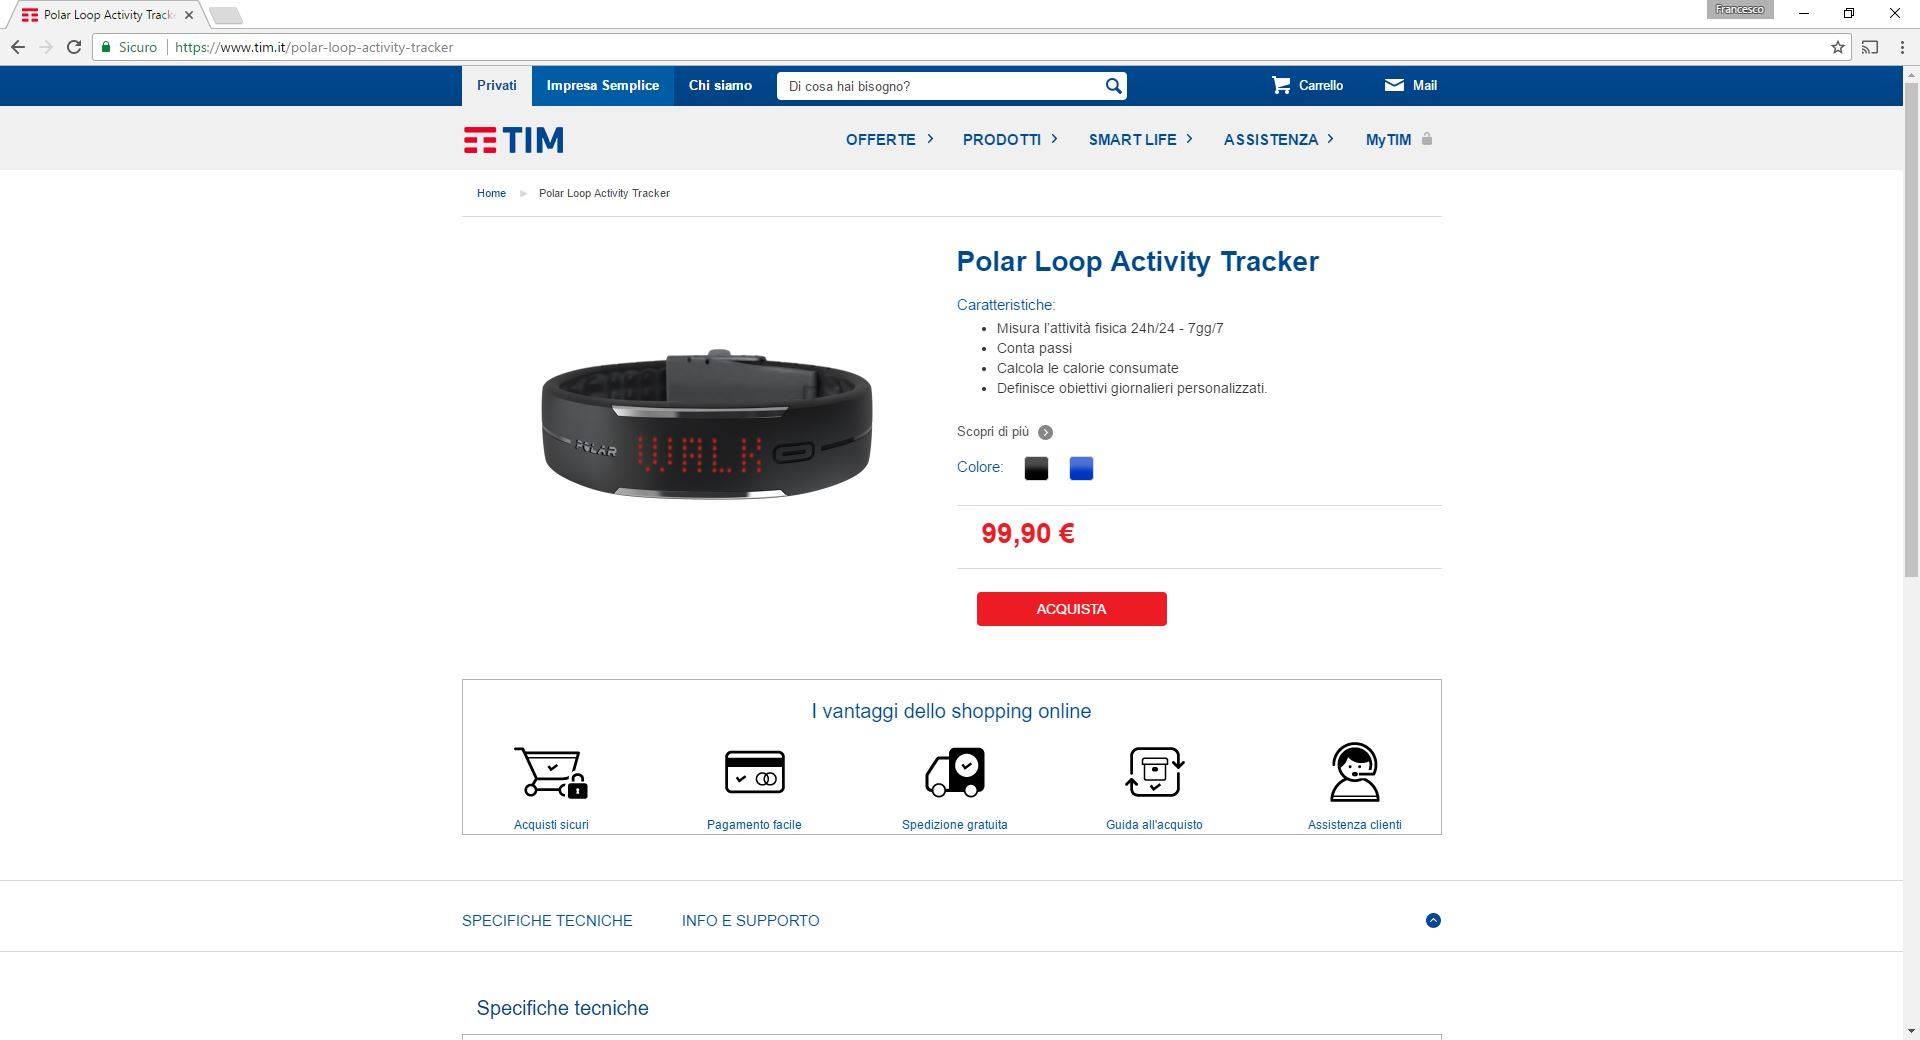
\includegraphics[width=\textwidth]{Screenshot/loop.jpg}
\end{center}
\vspace{1cm}

	\paragraph*{Content heuristics \\ Text}
	\begin{itemize}
		\item accuracy: satisfied
		\item currency: \textcolor{red}{severely violated}\\
		the user cannot know if the page is updated
		\item coverage: satisfied
		\item content objectivity: satisfied
		\item authority: satisfied
		\item conciseness: satisfied		
	\end{itemize}
	
	\paragraph*{General communication quality}
	\begin{itemize}
		\item text errors: satisfied
		\item multimedia consistency: satisfied
	\end{itemize}
	
	\paragraph*{Navigation heuristics \\ Navigation within a topic}
	\begin{itemize}
		\item segmentation: satisfied\\
		the information of the topic are organized in sub-sections on the same page 
	\end{itemize}	
	
	\paragraph*{Navigation within a transition}
	\begin{itemize}
		\item transition list: satisfied
	\end{itemize}
	
	\paragraph*{Navigation within a group of topics}
	\begin{itemize}
		\item introduction list: n/a
		\item group navigation: n/a
	\end{itemize}
	
	\paragraph*{Backward navigation}
	\begin{itemize}
		\item go back: \textcolor{red}{severely violated}\\
		there is no "go back" functionality, the user can go to the homepage through the TIM logo or repeat the steps by clicking "SMART LIFE"
	\end{itemize}
	
	\paragraph*{Overall navigation}
	\begin{itemize}
		\item landmarks: satisfied
		\item link consistency: satisfied
		\item orientation clues: \textcolor{red}{partially violated}\\
		\item orientation clues - topic: satisfied
		\item group orientation clues: n/a
		\item transition orientation clues: satisfied
	\end{itemize}	
	
	\paragraph*{Visual and semantic heuristics \\ Overall graphic design }
	\begin{itemize}
		\item visual identity: satisfied
		\item chromatic code consistency: satisfied
		\item background contrast:satisfied
		\item font size: satisfied
		\item font colour: satisfied
		\item font type: satisfied
		\item anchor identity: satisfied
		\item anchor states: satisfied
		\item icon consistency: satisfied
	\end{itemize}
	
	\paragraph*{Page layout}
	\begin{itemize}
		\item visual proximity: satisfied
		\item layout conventions: satisfied
		\item semiotics: satisfied
	\end{itemize}	
	
	\paragraph*{Cognitive heuristics \\ Single page}
	\begin{itemize}
		\item information overload: satisfied
	\end{itemize}	

	\paragraph*{Information architecture}
	\begin{itemize}
		\item classification adequacy within group of topics: satisfied
		\item website mental map: satisfied
	\end{itemize}
\newpage

%------------------------------------------------------------------------------------------------------

\item Report on \url{https://www.tim.it/prodotti/tv-e-smart-living/samsung-gear-fit}

\begin{center}
	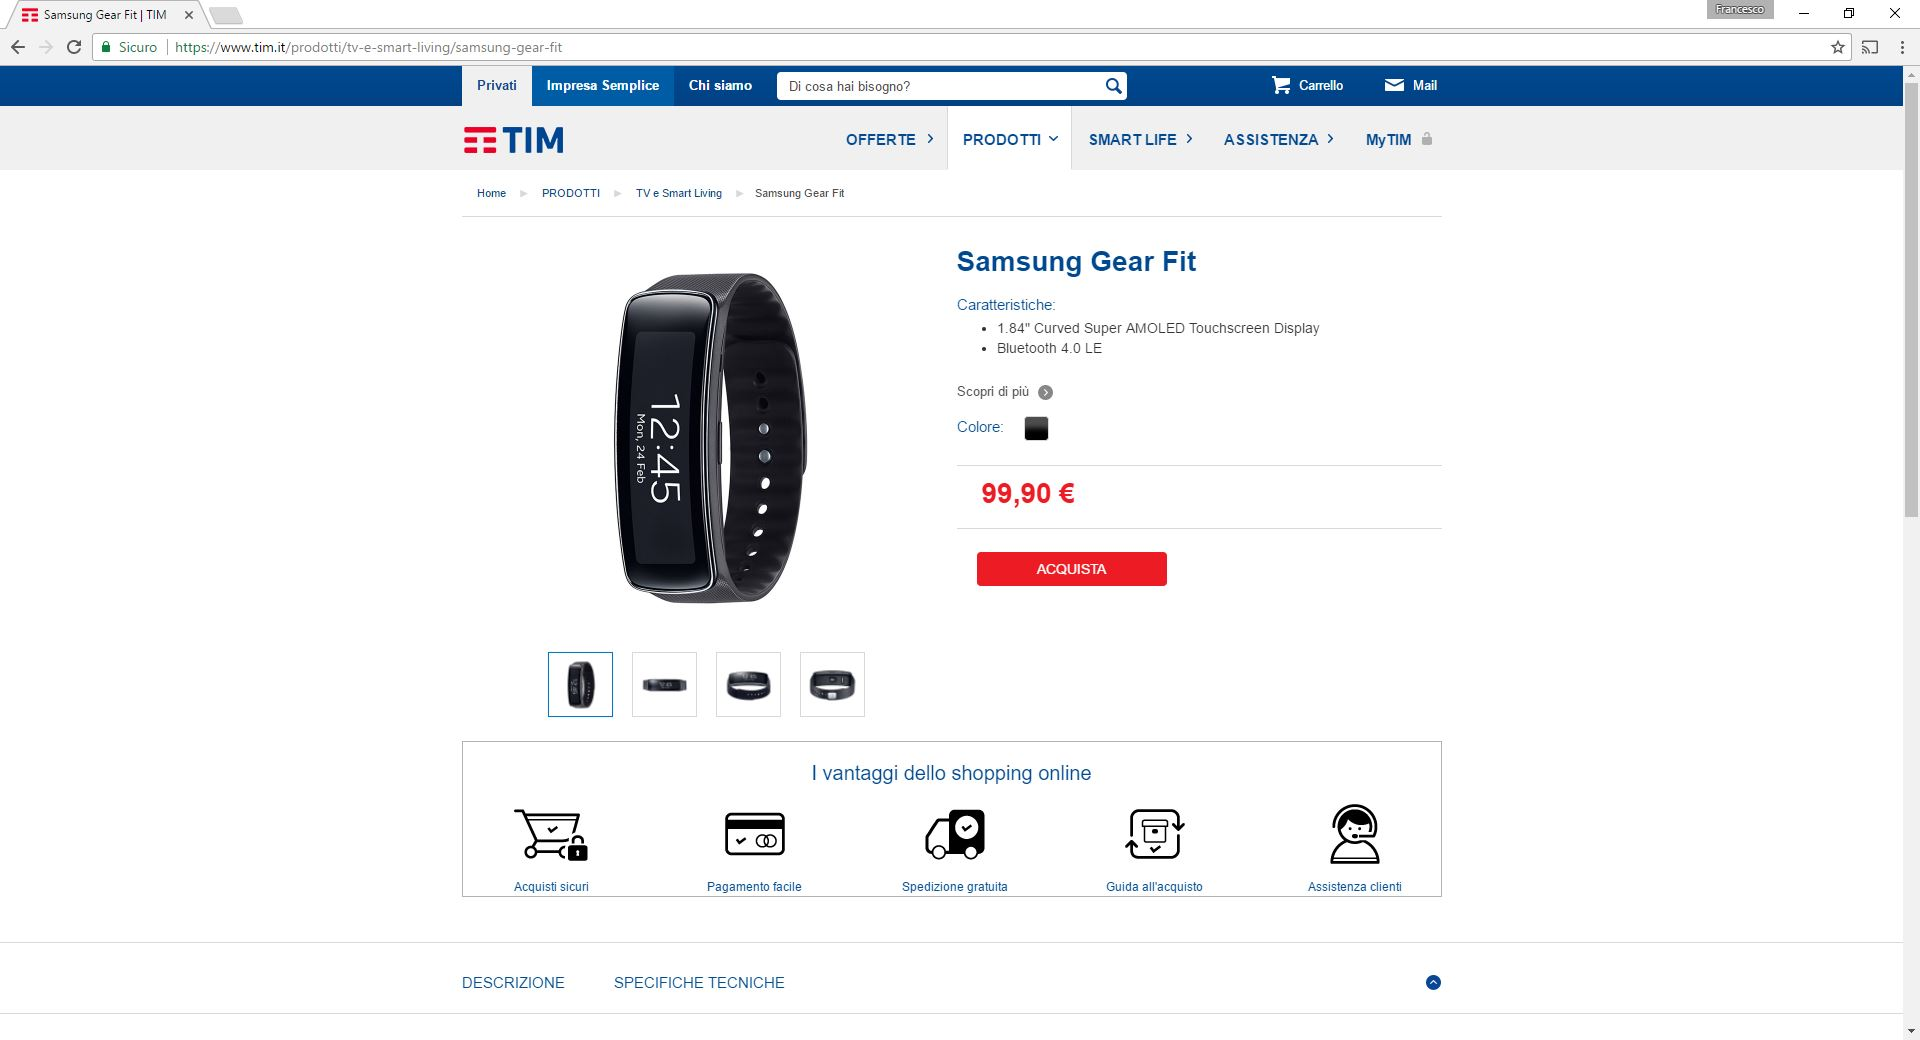
\includegraphics[width=\textwidth]{Screenshot/gear.jpg}
\end{center}
\vspace{1cm}

	\paragraph*{Content heuristics \\ Text}
	\begin{itemize}
		\item accuracy: satisfied
		\item currency: \textcolor{red}{severely violated}\\
		the user cannot know if the page is updated
		\item coverage: satisfied
		\item content objectivity: satisfied
		\item authority: satisfied
		\item conciseness: satisfied		
	\end{itemize}

	\paragraph*{General communication quality}
	\begin{itemize}
		\item text errors: satisfied
		\item multimedia consistency: satisfied
	\end{itemize}

	\paragraph*{Navigation heuristics \\ Navigation within a topic}
	\begin{itemize}
		\item segmentation: satisfied\\
		the information of the topic are organized in sub-sections on the same page
	\end{itemize}	

	\paragraph*{Navigation within a transition}
	\begin{itemize}
		\item transition list: satisfied
	\end{itemize}

	\paragraph*{Navigation within a group of topics}
	\begin{itemize}
		\item introduction list: n/a
		\item group navigation: n/a
	\end{itemize}

	\paragraph*{Backward navigation}
	\begin{itemize}
		\item go back: \textcolor{red}{severely violated}\\
		there is no "go back" functionality, the user can go to the homepage through the TIM logo or repeat the steps by clicking "SMART LIFE"
	\end{itemize}

	\paragraph*{Overall navigation}
	\begin{itemize}
		\item landmarks: satisfied
		\item link consistency: satisfied
		\item orientation clues: satisfied
		\item orientation clues - topic: satisfied
		\item group orientation clues: satisfied
		\item transition orientation clues: satisfied
	\end{itemize}	

	\paragraph*{Visual and semantic heuristics \\ Overall graphic design }
	\begin{itemize}
		\item visual identity: satisfied (the colors represents the logo of the company)
		\item chromatic code consistency: satisfied
		\item background contrast:satisfied
		\item font size: satisfied
		\item font colour: satisfied
		\item font type: satisfied
		\item anchor identity: satisfied
		\item anchor states: satisfied
		\item icon consistency: satisfied
	\end{itemize}

	\paragraph*{Page layout}
	\begin{itemize}
		\item visual proximity: satisfied
		\item layout conventions: satisfied
		\item semiotics: satisfied
	\end{itemize}

	\paragraph*{Cognitive heuristics \\ Single page}
	\begin{itemize}
		\item information overload: satisfied
	\end{itemize}	

	\paragraph*{Information architecture}
	\begin{itemize}
		\item classification adequacy within group of topics: satisfied
		\item website mental map: satisfied
	\end{itemize}
\end{enumerate}
\section{Scenario 4 TODO}
Dalia has to buy a new smartphone. He loves the services that his provider offers and he knows he can buy a new phone on its website.

\begin{enumerate}
	\item He goes on \url{www.tim.it}
	\item He clicks on "PRODOTTI" \url{www.tim.it/prodotti}
	\item In the smartphone section he can choose between smartphone or iPhone. He clicks on "iPhone". \url{www.tim.it/prodotti/smartphone-e-telefoni/iphone}
	\item Alberto sees that there are no promotions on iPhone so he goes back by clicking on "PRODOTTI"
	\item There is a promotion on Samsung Galaxy S8. He clicks on "SCOPRI". \url{www.tim.it/prodotti/smartphone-e-telefoni/samsung-galaxy-s8}
	\item He looks for the price and the specs. Alberto is interested and he wants to buy this phone. He clicks on "ACQUISTA". He is redirected on the ecommerce website of TIM and purchase is continued through this site.
\end{enumerate}

\subsection{Results}
\begin{enumerate}
	
%------------------------------------------------------------------------------------------------------
	
\item Report on \url{www.tim.it}	
	\paragraph*{Content heuristics \\ Text}
	\begin{itemize}
		\item accuracy: satisfied
		\item currency: \textcolor{red}{severely violated}\\the user cannot know if the page is updated
		\item coverage: satisfied
		\item content objectivity: satisfied
		\item authority: satisfied
		\item conciseness: satisfied		
	\end{itemize}
	
	\paragraph*{General communication quality}
	\begin{itemize}
		\item text errors: satisfied
		\item multimedia consistency: satisfied
	\end{itemize}

	\paragraph*{Navigation heuristics \\ Navigation within a topic}
	\begin{itemize}
		\item segmentation: n/a
	\end{itemize}	
	
	\paragraph*{Navigation within a transition}
	\begin{itemize}
		\item transition list: n/a
	\end{itemize}
	
	\paragraph*{Navigation within a group of topics}
	\begin{itemize}
		\item introduction list: satisfied
		\item group navigation: satisfied
	\end{itemize}
	
	\paragraph*{Backward navigation}
	\begin{itemize}
		\item go back: n/a
	\end{itemize}
	
	\paragraph*{Overall navigation}
	\begin{itemize}
		\item landmarks: satisfied
		\item link consistency: satisfied
		\item orientation clues: satisfied
		\item orientation clues - topic: n/a
		\item group orientation clues: n/a
		\item transition orientation clues: n/a
	\end{itemize}	
	
	\paragraph*{Visual and semantic heuristics \\ Overall graphic design }
	\begin{itemize}
		\item visual identity: satisfied\\
		the palette represents the colors of the company logo
		\item chromatic code consistency: satisfied
		\item background contrast:satisfied
		\item font size: satisfied
		\item font colour: satisfied
		\item font type: satisfied
		\item anchor identity: satisfied
		\item anchor states: satisfied
		\item icon consistency: satisfied
	\end{itemize}
	
	\paragraph*{Page layout}
	\begin{itemize}
		\item visual proximity: satisfied
		\item layout conventions: satisfied
		\item semiotics: satisfied
	\end{itemize}	
	
	\paragraph*{Cognitive heuristics \\ Single page}
	\begin{itemize}
		\item information overload: \textcolor{orange}{partially violated}\\
		due to the number of services that the site offers, a novice could be overwhelmed by a lot of informations
	\end{itemize}	
	
	\paragraph*{Information architecture}
	\begin{itemize}
		\item classification adequacy within group of topics: satisfied
		\item website mental map: satisfied
	\end{itemize}

%------------------------------------------------------------------------------------------------------

\item Report on \url{www.tim.it/prodotti}
	\paragraph*{Content heuristics \\ Text}
	\begin{itemize}
		\item accuracy: satisfied
		\item currency: severely violated
		\item coverage: satisfied
		\item content objectivity: satisfied
		\item authority: satisfied
		\item conciseness: satisfied		
	\end{itemize}

	\paragraph*{General communication quality}
	\begin{itemize}
		\item text errors: satisfied
		\item multimedia consistency: satisfied
	\end{itemize}

	\paragraph*{Navigation heuristics \\ Navigation within a topic}
	\begin{itemize}
		\item segmentation: n/a
	\end{itemize}	
	
	\paragraph*{Navigation within a transition}
	\begin{itemize}
		\item transition list: n/a
	\end{itemize}
	
	\paragraph*{Navigation within a group of topics}
	\begin{itemize}
		\item introduction list: satisfied
		\item group navigation: satisfied
	\end{itemize}

	\paragraph*{Backward navigation}
	\begin{itemize}
		\item go back: \textcolor {orange}{partially violated}\\
		there isn't a "go back" functionality but the user can exploit the TIM logo to return to the homepage or select a position in the website structure path (Home $\triangleright$ PRODOTTI)
	\end{itemize}
	
	\paragraph*{Overall navigation}
	\begin{itemize}
		\item landmarks: satisfied
		\item link consistency: satisfied
		\item orientation clues: satisfied
		\item orientation clues - topic: n/a
		\item group orientation clues: satisfied
		\item transition orientation clues: n/a
	\end{itemize}	
	
	\paragraph*{Visual and semantic heuristics \\ Overall graphic design }
	\begin{itemize}
		\item visual identity: satisfied
		\item chromatic code consistency: satisfied
		\item background contrast:satisfied
		\item font size: satisfied
		\item font colour: satisfied
		\item font type: satisfied
		\item anchor identity: satisfied
		\item anchor states: satisfied
		\item icon consistency: satisfied
	\end{itemize}
	
	\paragraph*{Page layout}
	\begin{itemize}
		\item visual proximity: satisfied
		\item layout conventions: satisfied
		\item semiotics: satisfied
	\end{itemize}	
	
	\paragraph*{Cognitive heuristics \\ Single page}
	\begin{itemize}
		\item information overload: satisfied
	\end{itemize}	
	
	\paragraph*{Information architecture}
	\begin{itemize}
		\item classification adequacy within group of topics: satisfied
		\item website mental map: satisfied
	\end{itemize}

%------------------------------------------------------------------------------------------------------

\item Report on \url{www.tim.it/prodotti/smartphone-e-telefoni/iphone}
	\paragraph*{Content heuristics \\ Text}
	\begin{itemize}
		\item accuracy: satisfied
		\item currency: \textcolor{red}{severely violated}
		\item coverage: satisfied
		\item content objectivity: satisfied
		\item authority: satisfied
		\item conciseness: satisfied		
	\end{itemize}
	
	\paragraph*{General communication quality}
	\begin{itemize}
		\item text errors: satisfied
		\item multimedia consistency: satisfied
	\end{itemize}
	
	\paragraph*{Navigation heuristics \\ Navigation within a topic}
	\begin{itemize}
		\item segmentation: n/a
	\end{itemize}	
	
	\paragraph*{Navigation within a transition}
	\begin{itemize}
		\item transition list: n/a
	\end{itemize}
	
	\paragraph*{Navigation within a group of topics}
	\begin{itemize}
		\item introduction list: satisfied
		\item group navigation: satisfied
	\end{itemize}
	
	\paragraph*{Backward navigation}
	\begin{itemize}
		\item go back: \textcolor{red}{severely violated}\\
		there is no "go back" functionality, the user can go to the homepage through the TIM logo or repeat the steps by clicking "PRODOTTI"
	\end{itemize}
	
	\paragraph*{Overall navigation}
	\begin{itemize}
		\item landmarks: satisfied
		\item link consistency: satisfied
		\item orientation clues: \textcolor{red}{severely violated}\\
		the user cannot know where he is, there are no title nor path
		\item orientation clues - topic: n/a
		\item group orientation clues: satisfied
		\item transition orientation clues: n/a
	\end{itemize}	
	
	\paragraph*{Visual and semantic heuristics \\ Overall graphic design }
	\begin{itemize}
		\item visual identity: satisfied
		\item chromatic code consistency: satisfied
		\item background contrast:satisfied
		\item font size: satisfied
		\item font colour: satisfied
		\item font type: satisfied
		\item anchor identity: satisfied
		\item anchor states: satisfied
		\item icon consistency: satisfied
	\end{itemize}
	
	\paragraph*{Page layout}
	\begin{itemize}
		\item visual proximity: satisfied
		\item layout conventions: satisfied
		\item semiotics: satisfied
	\end{itemize}	
	
	\paragraph*{Cognitive heuristics \\ Single page}
	\begin{itemize}
		\item information overload: satisfied
	\end{itemize}	

	\paragraph*{Information architecture}
	\begin{itemize}
		\item classification adequacy within group of topics: satisfied
		\item website mental map: satisfied
	\end{itemize}

%------------------------------------------------------------------------------------------------------

\item Report on \url{www.tim.it/prodotti/smartphone-e-telefoni/samsung-galaxy-s8}
	\paragraph*{Content heuristics \\ Text}
	\begin{itemize}
		\item accuracy: satisfied
		\item currency: severely violated
		\item coverage: satisfied
		\item content objectivity: satisfied
		\item authority: satisfied
		\item conciseness: satisfied		
	\end{itemize}

	\paragraph*{General communication quality}
	\begin{itemize}
		\item text errors: satisfied
		\item multimedia consistency: satisfied
	\end{itemize}

	\paragraph*{Navigation heuristics \\ Navigation within a topic}
	\begin{itemize}
		\item segmentation: satisfied\\
		the information of the topic are organized in sub-sections on the same page
	\end{itemize}	

	\paragraph*{Navigation within a transition}
	\begin{itemize}
		\item transition list: satisfied
	\end{itemize}

	\paragraph*{Navigation within a group of topics}
	\begin{itemize}
		\item introduction list: n/a
		\item group navigation: n/a
	\end{itemize}

	\paragraph*{Backward navigation}
	\begin{itemize}
		\item go back: \textcolor{orange}{partially violated}
	\end{itemize}

	\paragraph*{Overall navigation}
	\begin{itemize}
		\item landmarks: satisfied
		\item link consistency: satisfied
		\item orientation clues: satisfied
		\item orientation clues - topic: satisfied
		\item group orientation clues: satisfied
		\item transition orientation clues: satisfied
	\end{itemize}	

	\paragraph*{Visual and semantic heuristics \\ Overall graphic design }
	\begin{itemize}
		\item visual identity: satisfied (the colors represents the logo of the company)
		\item chromatic code consistency: satisfied
		\item background contrast:satisfied
		\item font size: satisfied
		\item font colour: satisfied
		\item font type: satisfied
		\item anchor identity: satisfied
		\item anchor states: satisfied
		\item icon consistency: satisfied
	\end{itemize}

	\paragraph*{Page layout}
	\begin{itemize}
		\item visual proximity: satisfied
		\item layout conventions: satisfied
		\item semiotics: satisfied
	\end{itemize}

	\paragraph*{Cognitive heuristics \\ Single page}
	\begin{itemize}
		\item information overload: satisfied
	\end{itemize}	

	\paragraph*{Information architecture}
	\begin{itemize}
		\item classification adequacy within group of topics: satisfied
		\item website mental map: satisfied
	\end{itemize}
	\end{enumerate}

\appendix
\chapter{Appendix}
\section{Version History}
In the following are listed the differences between versions:
\begin{itemize}
	\item 1.0.0: first release
\end{itemize}
\end{document}
